\section{Trip attraction (Exercise 2.2)}\label{sec:trip-attraction}

\paragraph{Data.}
Employment: URSSAF private-sector salaried employees 2019~\cite{urssaf-employment}, as prepared in
\cref{sec:territorial-II} (link given there). Sensitivity and plausibility check: INSEE MOBPRO RP2019~\cite{insee-mobpro-2019},
\url{https://www.insee.fr/fr/statistiques/6456056}. Departures \Oi{}: \cref{sec:trip-production}.

\subsection{Total number of trips \texorpdfstring{$N$}{N} and arriving trips per municipality (2 points)}

\begin{qa}{Report on the value of $N$ that you have chosen. Plot on a map how many arriving trips have been generated
for each municipality in the study area.}
$0.7 \sum_j W_j = 0.7 \times 180{,}618 = 126{,}432.6$ and $0.7 \sum_i \Oi = 0.7 \times 291{,}949 = 204{,}364.5$. The
employment term is the minimum, so \textbf{\boldmath $N = 126{,}432.6 \approx 126{,}433$ trips}. The arriving trips
per municipality are mapped in \cref{fig:arrivals-map}: Caen receives the most (24{,}672 trips, 19.5\,\% of $N$),
and 55 municipalities without URSSAF employees receive none.
\end{qa}

\paragraph{Method.}
The number of trips arriving in zone $j$ is proportional to its employment $W_j$:
\begin{equation}\label{eq:attraction}
  \Dj = \frac{W_j}{\sum_{j'} W_{j'}}\; N .
\end{equation}
Not all commuters generated in \cref{sec:trip-production} stay within the study area, and not all employees come from
within it. Following the assignment, the total number of trips within the study area is therefore the minimum of
70\,\% of the total employment and 70\,\% of the originating trips:
\begin{equation}\label{eq:total-trips-N}
  N = \min\!\left(0.7 \sum_j W_j,\; 0.7 \sum_i \Oi\right).
\end{equation}

The zones are the \textbf{528 municipalities}, sorted by INSEE code. This is the zone order of the whole pipeline from
\cref{sec:trip-distribution} on. $\Oi$ is the number of trips of \cref{sec:trip-production}, summed over the IRIS of
each municipality. As employment $W_j$ we use the \textbf{URSSAF private-sector employees} of 2019
\cite{urssaf-employment}, prepared in \cref{sec:territorial-II}, as in the course notebook. URSSAF counts only private
salaried jobs (no civil servants, hospitals, self-employed persons or farmers). It covers 65\,\% of the jobs counted by
MOBPRO \cite{insee-mobpro-2019} in Calvados (\cref{sec:territorial-II-mobpro}). As a sensitivity analysis, we repeat
the computation with the MOBPRO jobs at the place of work. Municipalities with $W_j = 0$ get $\Dj = 0$.
\begin{lstlisting}[style=py]
COMMUTER_SHARE = 0.7

def attraction(W, O, share=COMMUTER_SHARE):
    # N = min(share * sum W, share * sum O) and D_j = W_j / sum W * N
    W = np.asarray(W, dtype=float)
    N = min(share * W.sum(), share * O.sum())
    D = W / W.sum() * N
    return N, D

O = O_by_municipality.to_numpy()                    # 528 municipalities, sorted by INSEE code
N, D = attraction(df_employment["employees"], O)     # URSSAF (main result)
N_mobpro, D_mobpro = attraction(df_employment["jobs_mobpro"], O)   # sensitivity
\end{lstlisting}

\paragraph{Result.}
The URSSAF data give $\sum_j W_j = 180{,}618$ employees, and \cref{sec:trip-production} gives $\sum_i \Oi = 291{,}949$
trips. Hence $0.7 \sum_j W_j = 126{,}432.6$ and $0.7 \sum_i \Oi = 204{,}364.5$. The \textbf{employment term is the
minimum}, and \textbf{\boldmath $N = 126{,}432.6 \approx 126{,}433$ trips}, which is 43.3\,\% of the generated trips. We expected the employment term to bind: URSSAF misses about a third of the
jobs, while the model of \cref{sec:trip-production} produces about one trip per employed resident.

\begin{figure}[H]
  \centering
  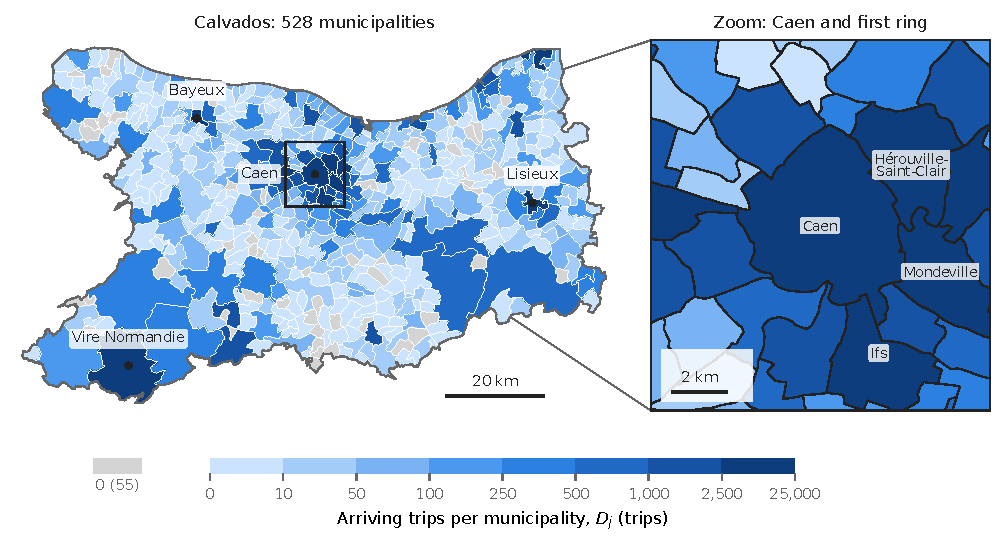
\includegraphics[width=\textwidth]{arrivals_map}
  \caption{Arriving trips \Dj{} per municipality, with URSSAF employment and $N = 126{,}433$. Grey: the 55
  municipalities without URSSAF employees ($\Dj = 0$). Right: zoom on Caen and its first ring. Data: URSSAF
  2019~\cite{urssaf-employment}, \cref{sec:trip-production}; IGN CONTOURS-IRIS 2021~\cite{ign-contours-iris};
  Lambert-93.}
  \label{fig:arrivals-map}
\end{figure}

The arrivals are much more concentrated than the departures (\cref{fig:arrivals-map}). Caen receives 24{,}672 trips
(19.5\,\% of $N$), followed by H\'erouville-Saint-Clair (7{,}783), Mondeville (7{,}350), Vire Normandie (6{,}278) and
Lisieux (5{,}795). These five municipalities receive 41.0\,\% of all trips, and the 30 largest receive 75.5\,\%. The
median is only 11 trips. Caen and its first ring form one dark block on the map. Bayeux, Lisieux, Vire Normandie,
Falaise and the coastal towns of Honfleur and Deauville are isolated dark spots. Most rural municipalities receive fewer
than 50 trips. The large rural \emph{communes nouvelles}, which have the highest production per IRIS
(\cref{fig:trips-per-iris-map}), are only mid-range here: they have many residents but few private jobs.
\textbf{55 municipalities have no URSSAF employee and receive no trip}. 10 of them have no URSSAF record at all, and 45
have a record with 0 employees. They are small villages: MOBPRO counts only 1{,}073 jobs in all of them together
(0.4\,\% of all jobs).

\paragraph{Sensitivity: MOBPRO jobs instead of URSSAF.}
With the MOBPRO jobs (all employed persons, at the place of work), $\sum_j W_j = 275{,}908$, so
$0.7 \sum_j W_j = 193{,}135$. This is still below $0.7 \sum_i \Oi = 204{,}365$, so \textbf{the employment term binds in
both variants}, but $N$ is 1.53 times larger (\cref{tab:attraction-sensitivity}). The spatial pattern is similar: the
\Dj{} of the two variants correlate at $r = 0.971$ ($0.969$ without Caen). The rank correlation is only 0.862, because
small municipalities with few private jobs change rank. The main difference is the public sector. With MOBPRO, Caen
receives 26.6\,\% of the trips instead of 19.5\,\%. With URSSAF, Caen, Bayeux and Lisieux (administration, hospitals,
schools) get only 48--61\,\% of their MOBPRO value. Private employment zones such as Mondeville and Bretteville-sur-Odon
get 7--31\,\% more.

\begin{table}[H]
  \centering
  \caption{Total number of trips $N$ with two sources for the employment $W_j$ (URSSAF private-sector employees,
  MOBPRO jobs). In both cases the employment term of \cref{eq:total-trips-N} is the minimum. $\Dj = 0$: number of
  municipalities without arrivals; Caen: share of $N$ that arrives in Caen.}
  \label{tab:attraction-sensitivity}
  \begin{tabular}{@{}lrrrrrr@{}}
    \toprule
    $W_j$ & $\sum_j W_j$ & $0.7 \sum_j W_j$ & $0.7 \sum_i \Oi$ & $N$ & $\Dj = 0$ & Caen \\
    \midrule
    URSSAF (used) & 180{,}618 & \textbf{126{,}433} & 204{,}365 & \textbf{126{,}433} & 55 & 19.5\,\% \\
    MOBPRO jobs & 275{,}908 & \textbf{193{,}135} & 204{,}365 & 193{,}135 & 7 & 26.6\,\% \\
    \bottomrule
  \end{tabular}
\end{table}

\subsection{Scaling the demand \texorpdfstring{$\Oprime$}{O'} (preparation for Exercise 2.3)}

\paragraph{Method.}
In a balanced model, the total number of originating trips must equal the total number of arriving trips. The demand
of \cref{sec:trip-production} is therefore scaled proportionally to the total $N$:
\begin{equation}\label{eq:scaling}
  \Oprime = N\, \frac{\Oi}{\sum_{i'} O_{i'}} .
\end{equation}
By construction, $\sum_i \Oprime = \sum_j \Dj = N$. Each municipality keeps its share of the trips, so \Oprime{} has
the same spatial pattern as \Oi{}.
\begin{lstlisting}[style=py]
O_scaled = N * O / O.sum()                       # factor N / sum(O) = 0.4331
assert np.isclose(O_scaled.sum(), D.sum())       # both equal N

zones = gdf_municipalities[["municipality_id", "name", "geometry"]].copy()
zones["O"], zones["D"] = O_scaled, D
write_zones(zones)          # checks the contract, writes data/processed/zones.parquet
\end{lstlisting}

\paragraph{Result.}
The scaling factor is $N / \sum_i \Oi = 0.4331$. Caen, for example, goes from 40{,}937 to 17{,}728 departures.
$\sum_i \Oprime = \sum_j \Dj = 126{,}432.6$; the difference is 0.0, also after the file has been written and read back.
Since \Oprime{} and \Dj{} now have the same total, they can be compared per municipality (\cref{fig:net-balance-map}).
471 municipalities have more departures than arrivals, and 57 have more arrivals. The largest surpluses of arrivals
are Caen ($-6{,}944$), Mondeville ($-5{,}517$), H\'erouville-Saint-Clair ($-3{,}947$), Vire Normandie ($-3{,}556$) and
Lisieux ($-2{,}504$). The largest surpluses of departures are rural \emph{communes nouvelles}, led by Souleuvre en
Bocage ($+1{,}057$) and M\'ezidon Vall\'ee d'Auge ($+980$). These are the same five municipalities as the largest net
outflows of the scaled comparison in \cref{sec:territorial-II-difference}. This is the commuting pattern that the
gravity model of \cref{sec:trip-distribution} has to reproduce.

\begin{figure}[H]
  \centering
  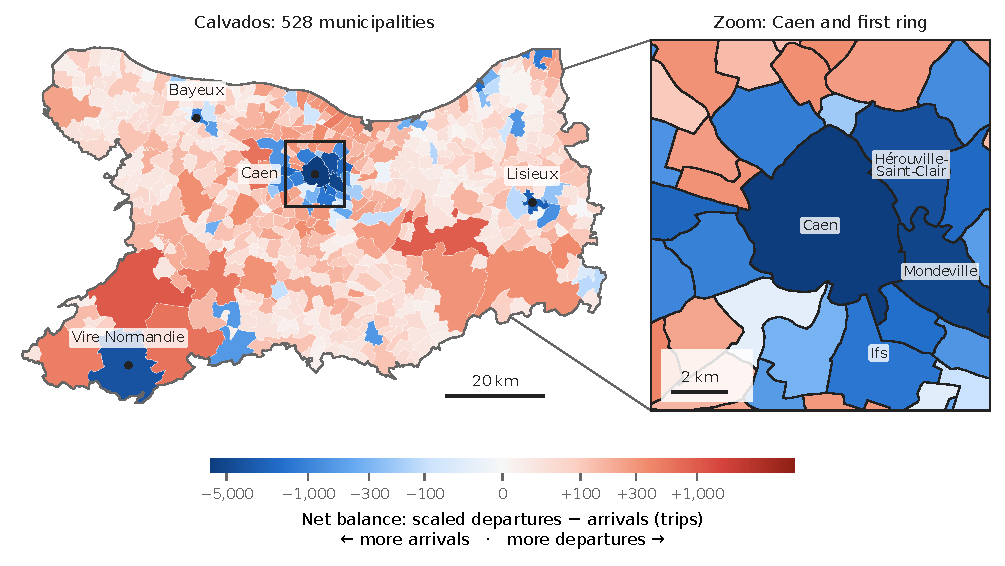
\includegraphics[width=\textwidth]{net_balance_map}
  \caption{Net balance $\Oprime - \Dj$ per municipality (scaled departures minus arrivals, both summing to $N$). Red:
  more departures (residential); blue: more arrivals (employment centres). The colour scale is linear within
  $\pm 100$ trips and logarithmic beyond, as in \cref{sec:territorial-II}.}
  \label{fig:net-balance-map}
\end{figure}

\paragraph{Hand-off file.}
\Oprime{} and \Dj{}, together with the municipality geometry, form the hand-off file
\code{data/processed/zones.parquet}: 528 rows sorted by INSEE code, with the columns \code{municipality\_id},
\code{name}, \code{geometry} (EPSG:2154), \code{O}~$=\Oprime$ and \code{D}~$=\Dj$. It is the only interface to the second part of the project
(\crefrange{sec:trip-distribution}{sec:routing}). The file is written by a function that checks the
contract, and it passes the check after being read back: unique codes identical to the municipality boundaries, no
missing or negative values, and $\sum O = \sum D = N$.

\subsection{Plausibility check with commuting data}\label{sec:trip-attraction-plausibility}

There is no ``true'' value of \Dj{}, but MOBPRO RP2019 \cite{insee-mobpro-2019} counts the real commuters
(\cref{tab:attraction-plausibility}). \textbf{255{,}249 persons} both live and work in Calvados: 171{,}986 between
different municipalities and 83{,}263 within their own municipality. This is 92\,\% of the employed residents and of
the jobs, not 70\,\%. Our $N = 126{,}433$ is therefore only \textbf{49.5\,\% of the real number} (73.5\,\% of the
commuters between different municipalities). With the MOBPRO jobs it would be 75.7\,\%.

\begin{table}[H]
  \centering
  \caption{Scaled departures \Oprime{} and arrivals \Dj{} compared with MOBPRO RP2019, Calvados: ratio of the totals,
  and Pearson ($r$) and Spearman ($\rho$) correlation over the 528 municipalities. ``Within Calvados'': commuters with
  home and work in the department.}
  \label{tab:attraction-plausibility}
  \begin{tabular}{@{}llrrrrr@{}}
    \toprule
    Model & Reference (MOBPRO) & Total & Ratio & $r$ & $r$ excl.\ Caen & $\rho$ \\
    \midrule
    \Dj{} & Jobs at the place of work & 275{,}908 & 0.458 & 0.971 & 0.969 & 0.862 \\
    \Dj{} & Arrivals within Calvados & 255{,}249 & 0.495 & 0.969 & 0.970 & 0.857 \\
    \Oprime{} & Employed residents & 277{,}131 & 0.456 & 0.9995 & 0.9974 & 0.997 \\
    \Oprime{} & Departures within Calvados & 255{,}249 & 0.495 & 0.9992 & 0.9957 & 0.991 \\
    \bottomrule
  \end{tabular}
\end{table}

The spatial pattern is plausible. \Oprime{} follows the real departures almost exactly ($r = 0.9992$). \Dj{} follows
the real arrivals well ($r = 0.969$), but less closely. The five largest real destinations are also the five largest
\Dj{}, and they receive 43.8\,\% of the real arrivals against 41.0\,\% of $D$. Within this group, Caen gets 19.5\,\% of
$D$ but 27.1\,\% of the real arrivals. Mondeville (5.8\,\% against 3.7\,\%), Vire Normandie and
H\'erouville-Saint-Clair are over-weighted, while Lisieux is about right.

For the simulation in \cref{sec:disaggregation,sec:routing}, this means that the model produces about 126{,}000
home-to-work trips, \textbf{about half of the real number}. Traffic volumes on the network will be underestimated by
about a factor of two, and trips into Caen will be too few compared with the private employment zones around it.

\paragraph{Problems encountered.}
\begin{itemize}
  \item \emph{URSSAF covers only private salaried jobs.} The total employment is 65\,\% of the MOBPRO jobs. As a result,
  the employment term determines $N$, which is only 43\,\% of the generated trips and half of the real commuters.
  Towns with many public jobs, Caen above all, get too small a share of the arrivals. We keep URSSAF, as in the course
  notebook and \cref{sec:territorial-II}, and report the MOBPRO variant as a sensitivity analysis.
  \item \emph{Municipalities without URSSAF employees.} 55 municipalities have $W_j = 0$ and therefore $\Dj = 0$. They
  have only 0.4\,\% of the MOBPRO jobs, so the effect on the result is negligible. In \cref{sec:trip-distribution} no
  trip ends there, not even within the municipality, but their residents still depart.
  \item \emph{The 70\,\% rule.} In Calvados, 92\,\% of the employed residents also work in the department. The factor
  0.7 is therefore conservative, and together with the URSSAF coverage it halves the number of trips. We apply the
  formula of the assignment and document the difference above.
\end{itemize}
